\documentclass[11pt]{article}

\newcommand{\yourname}{Gabriel Peter}
\newcommand{\yourcollaborators}{}

\def\comments{0}

%format and packages

%\usepackage{algorithm, algorithmic}
\usepackage{algpseudocode}
\usepackage{amsmath, amssymb, amsthm}
\usepackage{enumerate}
\usepackage{enumitem}
\usepackage{listings}
\usepackage{framed}
\usepackage{verbatim}
\usepackage[margin=1.0in]{geometry}
\usepackage{microtype}
\usepackage{kpfonts}
\usepackage{palatino}
	\DeclareMathAlphabet{\mathtt}{OT1}{cmtt}{m}{n}
	\SetMathAlphabet{\mathtt}{bold}{OT1}{cmtt}{bx}{n}
	\DeclareMathAlphabet{\mathsf}{OT1}{cmss}{m}{n}
	\SetMathAlphabet{\mathsf}{bold}{OT1}{cmss}{bx}{n}
	\renewcommand*\ttdefault{cmtt}
	\renewcommand*\sfdefault{cmss}
	\renewcommand{\baselinestretch}{1.06}
\usepackage[usenames,dvipsnames]{xcolor}
\definecolor{DarkGreen}{rgb}{0.15,0.5,0.15}
\definecolor{DarkRed}{rgb}{0.6,0.2,0.2}
\definecolor{DarkBlue}{rgb}{0.2,0.2,0.6}
\definecolor{DarkPurple}{rgb}{0.4,0.2,0.4}
\usepackage[pdftex]{hyperref}
\hypersetup{
	linktocpage=true,
	colorlinks=true,				% false: boxed links; true: colored links
	linkcolor=DarkBlue,		% color of internal links
	citecolor=DarkBlue,	% color of links to bibliography
	urlcolor=DarkBlue,		% color of external links
}

\usepackage[boxruled,vlined,nofillcomment]{algorithm2e}
	\SetKwProg{Fn}{Function}{\string:}{}
	\SetKwFor{While}{While}{}{}
	\SetKwFor{For}{For}{}{}
	\SetKwIF{If}{ElseIf}{Else}{If}{:}{ElseIf}{Else}{:}
	\SetKw{Return}{Return}

\usepackage{tikz}
	\usetikzlibrary{positioning}
	\definecolor{processblue}{cmyk}{0.96,0,0,0}
    \usetikzlibrary{matrix,arrows}

	

%enclosure macros
\newcommand{\paren}[1]{\ensuremath{\left( {#1} \right)}}
\newcommand{\bracket}[1]{\ensuremath{\left\{ {#1} \right\}}}
\renewcommand{\sb}[1]{\ensuremath{\left[ {#1} \right\]}}
\newcommand{\ab}[1]{\ensuremath{\left\langle {#1} \right\rangle}}

%probability macros
\newcommand{\ex}[2]{{\ifx&#1& \mathbb{E} \else \underset{#1}{\mathbb{E}} \fi \left[#2\right]}}
\newcommand{\pr}[2]{{\ifx&#1& \mathbb{P} \else \underset{#1}{\mathbb{P}} \fi \left[#2\right]}}
\newcommand{\var}[2]{{\ifx&#1& \mathrm{Var} \else \underset{#1}{\mathrm{Var}} \fi \left[#2\right]}}


%useful CS macros
\newcommand{\poly}{\mathrm{poly}}
\newcommand{\polylog}{\mathrm{polylog}}
\newcommand{\zo}{\{0,1\}}
\newcommand{\pmo}{\{\pm1\}}

\newcommand{\getsr}{\gets_{\mbox{\tiny R}}}
\newcommand{\card}[1]{\left| #1 \right|}
\newcommand{\set}[1]{\left\{#1\right\}}
\newcommand{\negl}{\mathrm{negl}}
\newcommand{\eps}{\varepsilon}
\DeclareMathOperator*{\argmin}{arg\,min}
\DeclareMathOperator*{\argmax}{arg\,max}
\newcommand{\eqand}{\qquad \textrm{and} \qquad}
\newcommand{\ind}[1]{\mathbb{I}\{#1\}}
\newcommand{\sslash}{\ensuremath{\mathbin{/\mkern-3mu/}}}

%mathbb
\newcommand{\N}{\mathbb{N}}
\newcommand{\R}{\mathbb{R}}
\newcommand{\Z}{\mathbb{Z}}
%mathcal
\newcommand{\cA}{\mathcal{A}}
\newcommand{\cB}{\mathcal{B}}
\newcommand{\cC}{\mathcal{C}}
\newcommand{\cD}{\mathcal{D}}
\newcommand{\cE}{\mathcal{E}}
\newcommand{\cF}{\mathcal{F}}
\newcommand{\cL}{\mathcal{L}}
\newcommand{\cM}{\mathcal{M}}
\newcommand{\cO}{\mathcal{O}}
\newcommand{\cP}{\mathcal{P}}
\newcommand{\cQ}{\mathcal{Q}}
\newcommand{\cR}{\mathcal{R}}
\newcommand{\cS}{\mathcal{S}}
\newcommand{\cU}{\mathcal{U}}
\newcommand{\cV}{\mathcal{V}}
\newcommand{\cW}{\mathcal{W}}
\newcommand{\cX}{\mathcal{X}}
\newcommand{\cY}{\mathcal{Y}}
\newcommand{\cZ}{\mathcal{Z}}

%theorem macros
\newtheorem{thm}{Theorem}
\newtheorem{lem}[thm]{Lemma}
\newtheorem{fact}[thm]{Fact}
\newtheorem{clm}[thm]{Claim}
\newtheorem{rem}[thm]{Remark}
\newtheorem{coro}[thm]{Corollary}
\newtheorem{prop}[thm]{Proposition}
\newtheorem{conj}[thm]{Conjecture}

\theoremstyle{definition}
\newtheorem{defn}[thm]{Definition}

\usepackage{mathtools}
\DeclarePairedDelimiter{\ceil}{\lceil}{\rceil}


\newcommand{\instructor}{Drew van der Poel}
\newcommand{\hwnum}{4}
\newcommand{\hwdue}{Saturday, June 12 at 11:59pm via \href{https://gradescope.com/courses/266585}{Gradescope}}

\theoremstyle{theorem}
\newtheorem{prob}{Problem}
\newtheorem{sol}{Solution}

\definecolor{cit}{rgb}{0.05,0.2,0.45} 
\newcommand{\solution}{\medskip\noindent{\color{DarkBlue}\textbf{Solution:}}}

\begin{document}
{\Large 
\begin{center}{CS3000: Algorithms \& Data} --- Summer I '21 --- \instructor \end{center}}
{\large
\vspace{10pt}
\noindent Homework~\hwnum \vspace{2pt}\\
Due~\hwdue}

\bigskip
{\large
\noindent Name: \yourname \vspace{2pt}\\ Collaborators: \yourcollaborators}

\vspace{15pt}
\begin{itemize}

\item Make sure to put your name on the first page.  If you are using the \LaTeX~template we provided, then you can make sure it appears by filling in the \texttt{yourname} command.

\item This assignment is due~\hwdue.  No late assignments will be accepted.  Make sure to submit something before the deadline.

\item Solutions must be typeset in \LaTeX.  If you need to draw any diagrams, you may draw them by hand as long as they are embedded in the PDF.  I recommend using the source file for this assignment to get started.

\item I encourage you to work with your classmates on the homework problems. \emph{If you do collaborate, you must write all solutions by yourself, in your own words.}  Do not submit anything you cannot explain.  Please list all your collaborators in your solution for each problem by filling in the \texttt{yourcollaborators} command.

\item Finding solutions to homework problems on the web, or by asking students not enrolled in the class is strictly forbidden.

\end{itemize}

\newpage



\begin{prob} Huffman Code Example (\emph{10 points})\end{prob}

Given the following alphabet $\Sigma=\{a,b,c,d,e,f,g\}$ and corresponding frequencies, use Huffman's algorithm to compute an optimal prefix-free code. Represent the prefix-free code as a binary tree, with either 0 or 1 on each edge. Compute the expected encoding length.


\begin{center}
\begin{tabular}{|l|c|c|c|c|c|c|c|}
\hline
Letter  & a & b & c & d & e & f & g \\
\hline
Frequency & 0.25 & 0.21 & 0.2 & 0.1 & 0.08 & 0.05 & 0.11 \\
\hline
\end{tabular}
\end{center}

\solution \\

ATTACHED AS IMG 1.

\newpage


\begin{prob} I wish I was a baller (\emph{32+4 points}) \end{prob}


As president of the Northeastern chapter of the Big Ballers Club, you need to staff a booth at this year's open house. The open house runs for the interval $[s,t]$.  There are $n$ volunteers, each of which is able to cover the booth for the interval $[s_i,t_i]$ ($i \in \{1, \dots, n\}$).  You need to select a set of volunteers $S \subseteq \{1,\dots,n\}$ to \emph{cover} the entire open house, meaning that $\bigcup_{i \in S} [s_i,t_i] \supseteq [s,t]$.  Equivalently, for every time $z \in [s,t]$, there is some volunteer $i \in S$ such that $z \in [s_i, t_i]$.  Each member will be paid for their services, but ironically the Big Ballers Club has very limited funds, so you need to ensure $|S|$ is as small as possible.

In this problem you will design an efficient greedy algorithm that takes as input the numbers $s,t,s_1,t_1,\dots,s_n,t_n$ and outputs a set $S$ that covers the open house and uses the minimum number of staffers.  The running time of your algorithm should be at most $O(n^2)$. You may assume that a solution exists.

\bigskip
The following is an example input with $9$ volunteers.  One optimal solution is $S = \{ 1,3,9 \}$.

\begin{center}
\includegraphics[width=5in]{hw4-fig1.jpg}
\end{center}

\begin{enumerate}[label=(\alph*)]


\item(\textbf{8 points}) Describe your algorithm in pseudocode. Provide a few sentences describing your algorithm.

\solution \\

\lstinputlisting[language=Python]{2_pseudo.py} 

The solution is rather simple:\\\\
First, there is a preprocessing step which map's the staff array elements to also consist of there original
index. This is done to ensure regardless of the array manipulation (foreshadow) the start and end times for a shift
correlate to the original index which is also their label.\\
Next, the code enters a loop which iterates over until a shift's endtime is past or equal to the overall booth's
endtime. Therefore, each iteration of this outer loop guarantees that we find a new shift to add to the optimal solution.\\
How do we find the next optimal shift? Well the internal code the iterates through all the members of the "still-available" staff
and uses a two part greedy rule to consider if they are an optimal addition:\\
Part 1: The next segment of this schedule must overlap with the previous, meaning that the new shift in consideration must have a start
-time before or equal to the previous shift's endtime. This was a strict rule in the problem as the station should never be unmanned.\\
Part 2: The solution should have the most distant end time if it supports Part 1. During part c, it is explained why this is essential.\\\\

After all available staff shifts are considered it adds the best one found to the solution and makes the new "latest start time possible" the newly found shift's endtime.
The cycle stops once a segment's shift surpasses the endtime needed for the booth, and the solution is sorted and printed...\\\\




\item (\textbf{4 points}) Analyze the running time of your algorithm.

\solution \\


The solution has a $o(n^2)$ because for each shift found in N iterations, it removes 1 element from the array, which means that only n-1 iterations are needed to find the next consecutive shift. 
We can remove the optimal shift because it can only be used once per solution, and can no longer be considered again.

$n + (n-1) + (n-2) + ... + (n-n) = n^2 - \sum_{i}^{n}i = n^2 - \frac{n^2+n}{2}$ (gauss) $ = \frac{n^2-n}{2} < O(n^2) = o(n^2)$


\emph{Keep in mind that the preprocessing step is only o(n) which is insignificant to the meat of the algothihm of $n^2$}

\item (\textbf{12 points}) Prove that your algorithm finds a set of volunteers $S$ of minimum size to cover the open house. 

\solution \\
In order to prove the correctness of this algorithm, I will base my explanation off the in-class proof of "Greedy stays ahead." in conjunction with the "exchange argument".

You need to take an optimal solution S. You can tell that this solution can grant $|S|$ positions, where $|S|$ is the minimum shifts you needs for a contigious schedule.

Then you take your solution G, which is greedy.

Now you say the first job you chose in G, this shift is `i` and the time spent is $[s_i,t_i]$. There is two possibility, either `i` is in S or it's not. If it's not by replacing
one job in S by `i` you get a better solution. BUT S is optimal so you can conclude that `i` is in S. 
% You can do the same kind of reasoning to prove that the time associed with `i` in S is .

% TODO which "Stays ahead" part
Then you do that for every element. And you'll conclude that the amount of shifts required earned is the same in G and in S. So G is optimal.

\emph{In a more informal view, part 1 of the greedy rule ensures shift overlap; therefore, we need simply need the longest segments with a shift duration of s-t.
Longer segments will allow for less small shifts as their domain takes more of the total booth time. In the inner loop, we only exchange if the resulting solution is better,
by the exchange argument if we continue this pattern the solution we receive that can no longer be exchanged for an even better one is now in the optimal solution.}


\item \textbf{[8 points]} In order to better your familiarity with greedy algorithms, we have created a hackerrank challenge (\href{www.hackerrank.com/cs3000-summer1-2021-programming-assignment-4}{www.hackerrank.com/cs3000-summer1-2021-programming-assignment-4}). Please implement your greedy strategy and submit it to the challenge. Your grade for this part will depend on (a) how many test cases your implementation passes and (b) actually implementing a greedy strategy (we will check!).

In order to allow for efficient grading, please write your hackerrank account below.

\solution \\
peter\_g

\item \textbf{[+4 points]}  Describe a greedy algorithm which solves this problem in $o(n^2)$ time. State and justify your runtime.

\solution \\

\#A allows for $o(n^2)$ because it also remove solutions that will now never be valid after finding the best consecutive segment.
This is because if we find a certain shift to have a valid start time, but end up not being the best solution with the longest endtime,
 the shift will never be considered again since the new start-time is beyond this stale shift's start-time. 
 A shift will never be considered twice if it got beat by a superior shift in length. This leaves a guaranteed runtime of $ \le O(n^2) = o(n^2)$

In fact, the previous explanation on 2b) already supports the algo to be $o(n^2)$ since $\frac{n^2-n}{2}$ satifies that asymptotic runtime.
However, taking out even more segments allows for even more optimization, in a real-world example.

\end{enumerate}

\newpage

\begin{prob} Total Weighted Finish Time (\emph{24 points})\end{prob}

A scheduler needs to determine an order in which a set of $n$ processes will be assigned to a processor. The $i$-th process requires $t_i$ units of time and has weight $w_i$. For a given schedule, define the finish time of process $i$ to be the time at which process $i$ is completed by the processor. (Assume that the processor starts processing the tasks at time 0.)

For example, consider 4 processes with $t_1 = 5, t_2 = 2, t_3 = 7, t_4 = 4$. And weights $w_1 = 1, w_2 = 3, w_3 = 2,$ and $w_4 = 2$. Consider the schedule 1,3,2,4. The finish time for process 1 is 5, for process 2 is $t_1 + t_3 + t_2 = 5 + 7 + 2 = 14$, for process 3 is $t_1 + t_3$ = 5 + 7 = 12, and for process 4 is $t_1 + t_3 + t_2 + t_4 = 5 + 7 + 2 + 4 = 18$. The total weighted finish time of the schedule is then $5*1 + 14*3 + 12*2 + 18*2 = 5 + 42 + 24 + 36 = 107$. 




\begin{enumerate}[label=(\alph*)]

\item \textbf{[10 points]} Give a greedy algorithm to determine a schedule that minimizes the total weighted finish time. (\textbf{Hint: } If you are stuck, trying figuring out a rule that \emph{always} works when $n=2$).

\solution \\ 

\lstinputlisting[language=Python]{3_pseudo.py} 

For this greedy algorithm we state a precedence of Maximum weights then minimum times.
 This is based on intuition, then later proof, that multiplicative weights are significant 
more expensive than additive times and should be placed first in the queue such that a high-weight process does not multiply the entire summation of previous process times.
However, if the multiplicate times are the same for two processes, then the one which takes less time should be placed first (explained in 3b)\\

\#1, As a pre-processing step, the labels, times, and weights of the processes are a mapped to a single n-sized list, X.
\\\\ \#2-\#5This lays the groud work for our algorithm. For each search of the next S schedule, we interate through the availble 
processes and find one with max\_w in order to queue that first. In order to consider ties of max weight. 
The sub\_solution is an array and holds all processes with the maximum weight so far.
If a process is found with an even higher weight, it demotes all the other proccesses and becomes the sole sub\_solution... etc.

\#6: The minimum time of all tied-weight processes is found, then added to the solution. This ends the inner for-loop and 
a new iteration for $S_{i+1}$ is run until $|S| = n$ where all entries are unique.


\item \textbf{[10 points]} Prove the correctness of your algorithm.

\solution \\

Let $a$ be a constant. Informally we can quickly conclude that when $n > 1 \rightarrow n * a \ge n + a$.\\
This asserts the multiplicative precedence in our greedy algorightm. Where S is the current time summation of the schedule,
$S_i * n \le S_{i+1,2,3,...} * n$. 

Now for why smaller $t_i$ priority is used to break ties: We know that $S_i$ has a smaller sum than $S_{i+1}$. 
This is because $t_i$ is included in $S_i,.. S_n$ (based on how it is calculated) so if we put the larger values in further in the queue, those "sums" are then
reduced as they contain less uses of the greate $t_i$ value. However, as asserted before, the weights are more influential (multiplicative) than the times to process (additive),
which is why they're not equal in greedy rule but sequential.

Now that we know this, our greedy rule will create an optimal solution because it will always choose the next 
consecutive solution that decreases the summation total where the highest $w_i$'s and then lowest $t_i$'s are always picked first.
Given that we cannot invert the scheduling an expect a solution less than or equal to the value. We know that
the greedy schedule is equal to the optimal schedule, and that greedy stay's ahead as it will always pick the best consecutive answer without ambiguity. 
This is essentially a rephrasing of the exchange argument which has already been formally proven in class and in \#2! which can be applied here.


\item \textbf{[4 points]}  Analyze the worst-case running time of your algorithm.

\solution

The runtime of this algorithm is $O(n^2)$:\\\\
\#1 runs `n` times, as one solution is found per interation and the Schedule needs to include all n processes.
\#4 run `n` times in order to find the best next process to schedule as well as \#6 to find the minimum item.
\\However, \#4 and \#6 are additive functions: so we simplify our expression $O(n(n+n)) = O(n(2n)) \rightarrow O(n^2)$.
\\\\Although unnessary, I can already see optimizations like adding all $sub\_sols$ elements first in sorted $t_i$ 
order since they are all guaranteed to be the next elements of max weight. etc.\\



\end{enumerate}








\newpage
\begin{prob}Graph Representations and Exploration (15 points)\end{prob}
This problem is about the following graph.  {\bf Tip:} Use the \LaTeX for rendering the graph as a starting point if your solutions involve drawing a graph.

\begin{figure}[h!]
\begin{center}
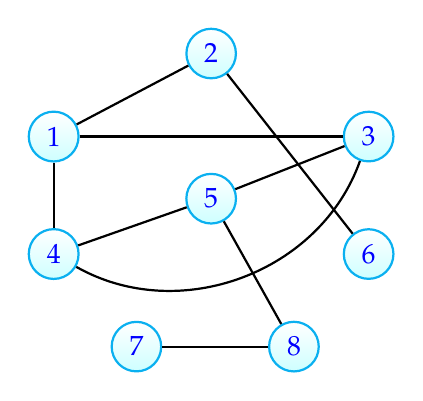
\begin{tikzpicture}[node distance = 1.0 cm and 2.0cm,on grid,
thick,state/.style ={circle,top color =white,bottom color = processblue!20,draw,processblue,text=blue,minimum width =.3 cm}]
\node[state] (a) {1};
\node[state] (b) [yshift = 30pt, right =of a] {2};
\node[state] (c) [yshift = -30pt, right =of b] {3};
\node[state] (d) [below =of a, yshift=-14pt] {4};
\node[state] (e) [yshift = 20pt, right =of d] {5};
\node[state] (f) [yshift = -20pt, right =of e] {6};
\node[state] (g) [below =of e, xshift=-27pt,yshift=-25pt] {7};
\node[state] (h) [right =of g] {8};
\path (a) edge [bend left = 0] (b) 
		edge [bend left = 0] (c) 
		edge (d);
\path (b) edge [bend left = 0] (f);
\path (c) edge [bend left = 0] (e);
\path (d) edge [bend right = 50] (c) 
		edge [bend left = 0] (e) 
		edge (d);
\path (e) edge [bend left = 0] (h);
\path (g) edge [bend left = 0] (h);
\end{tikzpicture}
\end{center}
\end{figure}

\begin{enumerate}[label=(\alph*)]
\item \textbf{[5 points]}  Draw the adjacency matrix of this graph.\footnote{{\bf Hint:} If drawing the matrix in latex, I recommend using the \texttt{tabular} or \texttt{matrix} environments.}

\solution \\

\begin{tabular}{||cccccccc||}
	1 & 2 & 3 & 4 & 5 & 6 & 7 & 8 \\
	\hline
	0 & 1 & 1 & 1 & 0 & 0 & 0 & 0 \\
	1 & 0 & 0 & 0 & 0 & 1 & 0 & 0 \\
	1 & 0 & 0 & 1 & 1 & 0 & 0 & 0 \\
	1 & 0 & 1 & 0 & 1 & 0 & 0 & 0 \\
	0 & 0 & 1 & 1 & 0 & 0 & 0 & 1 \\
	0 & 1 & 0 & 0 & 0 & 0 & 0 & 0 \\
	0 & 0 & 0 & 0 & 0 & 0 & 0 & 1 \\
	0 & 0 & 0 & 0 & 1 & 0 & 0 & 1 \\
\end{tabular}


\item \textbf{[5 points]}  Draw the adjacency list of this graph.

\solution \\
$[1] = \{2, 3, 4\}$ \\
$[2] = \{1, 6\}$ \\
$[3] = \{1, 4, 5\}$ \\
$[4] = \{1, 3, 5\}$ \\
$[5] = \{3, 4, 8\}$ \\
$[6] = \{2\}$ \\
$[7] = \{8\}$ \\
$[8] = \{5, 7\}$ \\

\item \textbf{[5 points]}  BFS this graph starting from the node $1$.  Always choose the lowest-numbered node next.  Draw the BFS tree and label each node with its distance from $1$.

\solution \\

ATTACHED AS IMG 2.

\end{enumerate}

\newpage

\begin{prob}Graph Properties (10 points)\end{prob}

\renewcommand{\deg}{\mathit{deg}}

Consider an undirected graph $G=(V,E)$. The {\em degree} of a vertex $v$ is the number of edges adjacent to $v$---that is, the number of edges of the form $(v,u) \in E$.  Recall the standard notational convention that $n = |V|$ and $m = |E|$.

 Prove by induction that the sum of the degrees of the vertices is equal to $2m$.

\solution \\\\
Base Case(s): \\
If $m = 0$, $\sum degrees(v) = 0$\\
If $m = 1$, $\sum degrees(v) = 2$\\
Suppose we have a graph G with $m$ edges where $m \ge 1$. 
By adding one edge by random, the resulting new 
graph now has $m+1$ edges, we shall name it H.
\\\\We will assume that our Inductive Hypothesis to be that 
$\sum degrees(v) = 2(m+1)$.\\\\
Through simple graph rules, 
we know that if we add a single edge, it must be connected by two vertices.
If those two vertices each acquire a degree of +1, then we know that 
the new summation of degrees is $ = 2m + 2$, which is equal to our IH through expression manipulation.
$\sum degrees(v) = 2(m+1) = 2m + 2$.\\\\Conclusion of proof.

\end{document}
